\section{Deployment and Integration}\label{sec:deployment-and-integration}
We decided to use GitHub Pages via an organization for distribution because it provides an easy way to access the
application for end users and simplifies the maintenance for developers.
The GitHub organization is located under: https://github.com/decibel-threshold-event-displayer
The application is deployed as a GitHub Page under: https://decibel-threshold-event-displayer.github.io/
The following list and the graphic~\ref{fig:deployment_flow} elaborates on the deployment workflow.

\begin{enumerate}
    \item A dev pushes or merges code to the main branch
    \item GitLab automatically mirrors the repository to GitHub
    \item GitHub deploys automatically to GitHub Pages
    \item {The Application is available under: \\
          https://decibel-threshold-event-displayer.github.io/}
\end{enumerate}

\begin{figure}[H]
    \centering
    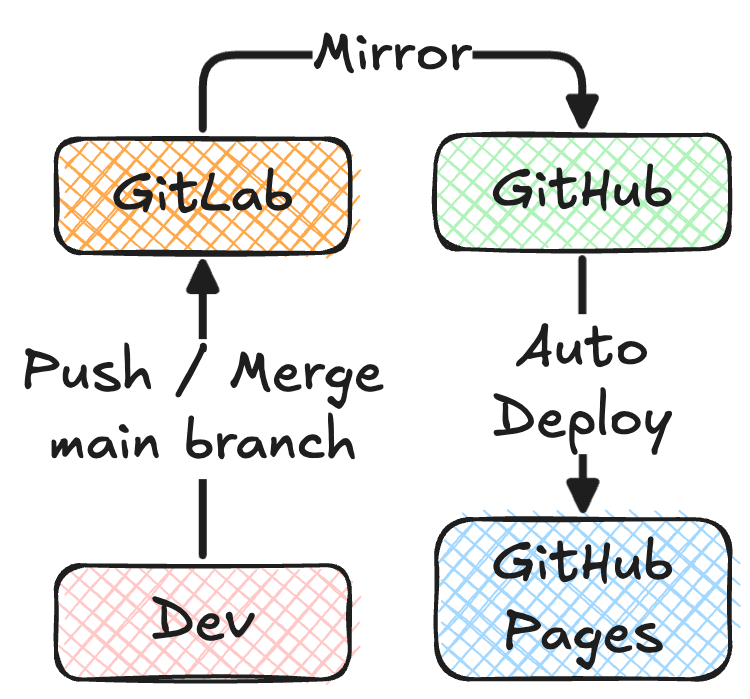
\includegraphics[width=0.5\textwidth]{../assets/deployment_and_distribution.png}
    \caption{Deployment Flow}\label{fig:deployment_flow}
\end{figure}

\subsection{Licensing}\label{subsec:licensing}
We already started to cover the topic in the evaluation under~\nameref{subsec:evaluation-license} and even though the project team tried to introduce the least amount of external dependencies,
the license still has to be revalidated at this point.
The following list contains all dependencies of the final application and their according license:
\begin{itemize}
    \item SwiftLaTeX: \href{https://github.com/SwiftLaTeX/SwiftLaTeX/blob/master/LICENSE}{SwiftLaTeX License}, \href{https://www.gnu.org/licenses/agpl-3.0.en.html}{GNU AFFERO GENERAL PUBLIC LICENSE}
    \item LaTeX: \href{https://www.latex-project.org/lppl.txt}{The LaTeX project public license} (GPL Compatible)
    \item TeXLive: \href{https://www.tug.org/texlive/copying.html}{TeX Live licensing, copying, and redistribution}, \href{https://www.tug.org/texlive/LICENSE.TL}{COPYING CONDITIONS FOR TeX Live} (GPL Compatible)
    \item pgfplots: \href{https://ctan.org/pkg/pgfplots}{https://ctan.org/pkg/pgfplots}, \href{https://www.gnu.org/licenses/gpl-3.0.en.html}{GNU General Public License, version 3 or newer}
    \item Bootstrap: \href{https://github.com/twbs/bootstrap/blob/main/LICENSE}{Bootstrap License}, \href{https://en.wikipedia.org/wiki/MIT_License}{MIT License} (GPL Compatible)
\end{itemize}

Considering all licenses of our dependencies are GPL based or GPL compatible,
we decided to use the following license for our application: \textbf{\href{https://www.gnu.org/licenses/gpl-3.0.en.html}{GPL-3.0 licence (FLOSS)}}

\subsection{Installation Manuel \& Script}\label{subsec:installation-manuel-and-script}
We are using a Makefile to automate the development setup, build and deploy the application to GitHub Pages.

\subsubsection{Development setup}\label{subsubsec:deployment-setup}
A local webserver is needed work on the application as some Browsers will not execute web workers on locally served files~\cite{stackoverflow_chrome_cant_load_web_worker}.
By default, the project uses the built-in webserver of Python 3.
Python 3 can be installed with the systems package manager or by downloading it from the official website: https://www.python.org/downloads/
Afterward the following command can be used to run the local webserver on http://0.0.0.0:8000/:

\begin{lstlisting}[caption={Makefile: Start local webserver},label={lst:makefile_start_local_webserver},language=Bash]
$ make dev
\end{lstlisting}

\subsubsection{Distribution}
The project and the repository is managed via the GitLab of BFH,
but we want to use GitHub pages to deploy and distribute our application,
the project team decided that we mirror the GitLab repository to GitHub:
\begin{itemize}
    \item \href{https://gitlab.ti.bfh.ch/decibel-threshold-event-displayer/decibel-threshold-event-displayer}{GitLab Repository}
    \item \href{https://github.com/decibel-threshold-event-displayer/decibel-threshold-event-displayer.github.io}{GitHub Repository}
\end{itemize}

\paragraph{Mirror setup:}
\begin{enumerate}
    \item Log into \href{https://gitlab.ti.bfh.ch}{gitlab.ti.bfh.ch}
    \item Navigate to the repository: \href{https://gitlab.ti.bfh.ch/decibel-threshold-event-displayer/decibel-threshold-event-displayer/}{GitLab Repository}
    \item Go to the repositories settings page: \href{https://gitlab.ti.bfh.ch/decibel-threshold-event-displayer/decibel-threshold-event-displayer/-/settings/repository}{Settings > Repository}
    \item Open the Tab ``Mirroring repositories``
    \item Click the button ``Add new``
    \item Fill the form as follows:
          \begin{itemize}
              \item Git repository URL: ssh://git@github.com/decibel-threshold-event-displayer/decibel-threshold-event-displayer.github.io.git
              \item Mirror direction: Pull
              \item Authentication method: SSH public key
              \item Username: github
              \item Mirror user: autofilled
              \item Overwrite diverged branches: Select
              \item Mirror branches > Mirror specific branches: main
          \end{itemize}
    \item Click the button ``Mirror repository``
    \item The first try will fail, as we have to add the public key generated by GitLab to the GitHub repository
    \item On the newly created entry, click the clipboard button ``Copy SSH public key`` (the public key is now in your clipboard)
    \item Keep the current GitLab tab open
    \item Log into \href{https://github.com/}{github.io} in a new tab
    \item Navigate to the repository: \href{https://github.com/decibel-threshold-event-displayer/decibel-threshold-event-displayer.github.io/}{GitHub Repository}
    \item Go to the repositories deploy keys page: \href{https://github.com/decibel-threshold-event-displayer/decibel-threshold-event-displayer.github.io/settings/keys}{Settings > Deploy Keys}
    \item Click the button ``Add deploy key``
    \item Fill the form as follows:
          \begin{itemize}
              \item Title: github
              \item Key: Copy the SSH public key from the clipboard
              \item Allow write access:
          \end{itemize}
    \item Click the button ``Add Key``
    \item Go back to the gitlab tab
    \item Click the reload button ``Update now``
    \item Wait until the process is finished
\end{enumerate}

\subsubsection{Build}
As we have only plain JavaScript files, we don't have a build step.

\subsubsection{Deploy}
As described above, we created a Mirror of this repository on GitHub.
Based on the following documentation, we configured GitHub to automatically deploy to GitHub Pages:
\href{https://docs.github.com/en/pages/getting-started-with-github-pages/creating-a-github-pages-site}{Creating a GitHub Pages site}

Further we had to add a configuration file under ``.github/workflows/static.yml`` and change value of ``path: \'./\'`` to ``path: \'./app\'``.
The initial file was generated by the following setup page:
\href{https://github.com/decibel-threshold-event-displayer/decibel-threshold-event-displayer.github.io/new/main?filename=.github%2Fworkflows%2Fstatic.yml&pages_workflow_template=pages%2Fstatic}{Repository > Settings > GitHub Pages > Static HTML > Configure}

\subsection{User Manual}\label{subsec:user-manuel}
The project team decided to not create an additional document for the user manual,
because all the necessary information for using the application are provided by following list of best practices:
\begin{itemize}
    \item Following common UI patterns
    \item Well-known form components
    \item Tooltips where needed
    \item Human-readable error messages
    \item About page with detailed technical information
\end{itemize}

